% TikZ Diagram: Causal multi-scale feature vector decomposition
% Color Rules: Raw window & output feature vector = White fill + Black stroke.
%              Middle feature blocks = Amber Accent fill + Amber stroke.

\documentclass[tikz,border=10pt]{standalone}
\usetikzlibrary{shapes.geometric, positioning, arrows.meta, chains, backgrounds}

\definecolor{neutralbg}{HTML}{F8FAFC}
\definecolor{neutralstroke}{HTML}{64748B}
\definecolor{neutraltext}{HTML}{0F172A}

\definecolor{accentbg}{HTML}{FEF3C7}
\definecolor{accentstroke}{HTML}{D97706}
\definecolor{accenttext}{HTML}{92400E}

\begin{document}
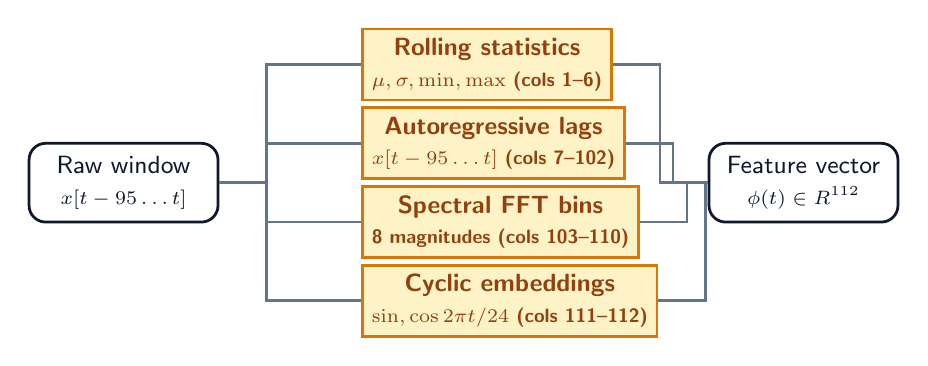
\begin{tikzpicture}[
    font=\sffamily\small,
    node distance=1.0cm and 1.2cm,
    wb_tensor/.style={rounded corners=6pt, draw=neutraltext, fill=white, text=neutraltext, minimum height=1.0cm, minimum width=2.4cm, align=center, line width=1.0pt},
    accent_op/.style={rectangle, draw=accentstroke, fill=accentbg, text=accenttext, minimum height=0.9cm, minimum width=3.0cm, align=center, line width=1.0pt, font=\sffamily\bfseries\small},
    arrow/.style={-{Stealth[scale=1.0]}, line width=1.0pt, draw=neutralstroke}
]

    % Raw stream input (White fill + Black stroke)
    \node[wb_tensor] (input) {Raw window\\{\scriptsize $x[t-95 \dots t]$}};

    % Middle transformation blocks (Golden Amber Accent)
    \node[accent_op, right=1.8cm of input, yshift=1.5cm] (b1) {Rolling statistics\\{\scriptsize $\mu, \sigma, \min, \max$ (cols 1--6)}};
    \node[accent_op, right=1.8cm of input, yshift=0.5cm] (b2) {Autoregressive lags\\{\scriptsize $x[t-95 \dots t]$ (cols 7--102)}};
    \node[accent_op, right=1.8cm of input, yshift=-0.5cm] (b3) {Spectral FFT bins\\{\scriptsize 8 magnitudes (cols 103--110)}};
    \node[accent_op, right=1.8cm of input, yshift=-1.5cm] (b4) {Cyclic embeddings\\{\scriptsize $\sin, \cos 2\pi t/24$ (cols 111--112)}};

    % Assembled output feature vector (White fill + Black stroke)
    \node[wb_tensor, right=6.2cm of input] (out) {Feature vector\\{\scriptsize $\phi(t) \in \mathbb{R}^{112}$}};

    % Bus Connector Manifold lines
    \draw[line width=1.0pt, draw=neutralstroke] (input.east) -- ++(0.6,0) |- (b1.west);
    \draw[line width=1.0pt, draw=neutralstroke] (input.east) -- ++(0.6,0) |- (b2.west);
    \draw[line width=1.0pt, draw=neutralstroke] (input.east) -- ++(0.6,0) |- (b3.west);
    \draw[line width=1.0pt, draw=neutralstroke] (input.east) -- ++(0.6,0) |- (b4.west);

    \draw[line width=1.0pt, draw=neutralstroke] (b1.east) -| ++(0.6,0) |- (out.west);
    \draw[line width=1.0pt, draw=neutralstroke] (b2.east) -| ++(0.6,0) |- (out.west);
    \draw[line width=1.0pt, draw=neutralstroke] (b3.east) -| ++(0.6,0) |- (out.west);
    \draw[line width=1.0pt, draw=neutralstroke] (b4.east) -| ++(0.6,0) |- (out.west);

\end{tikzpicture}
\end{document}
